\begin{figure}[h]
    \centering
    \begin{tikzpicture}[x=1cm,y=1cm]
      \def\height{9}
      
      \draw[white] (-\height/2,\height/2) rectangle (\height*1.1,-\height*1.5);
      
      \node (toppic) at (0,0) {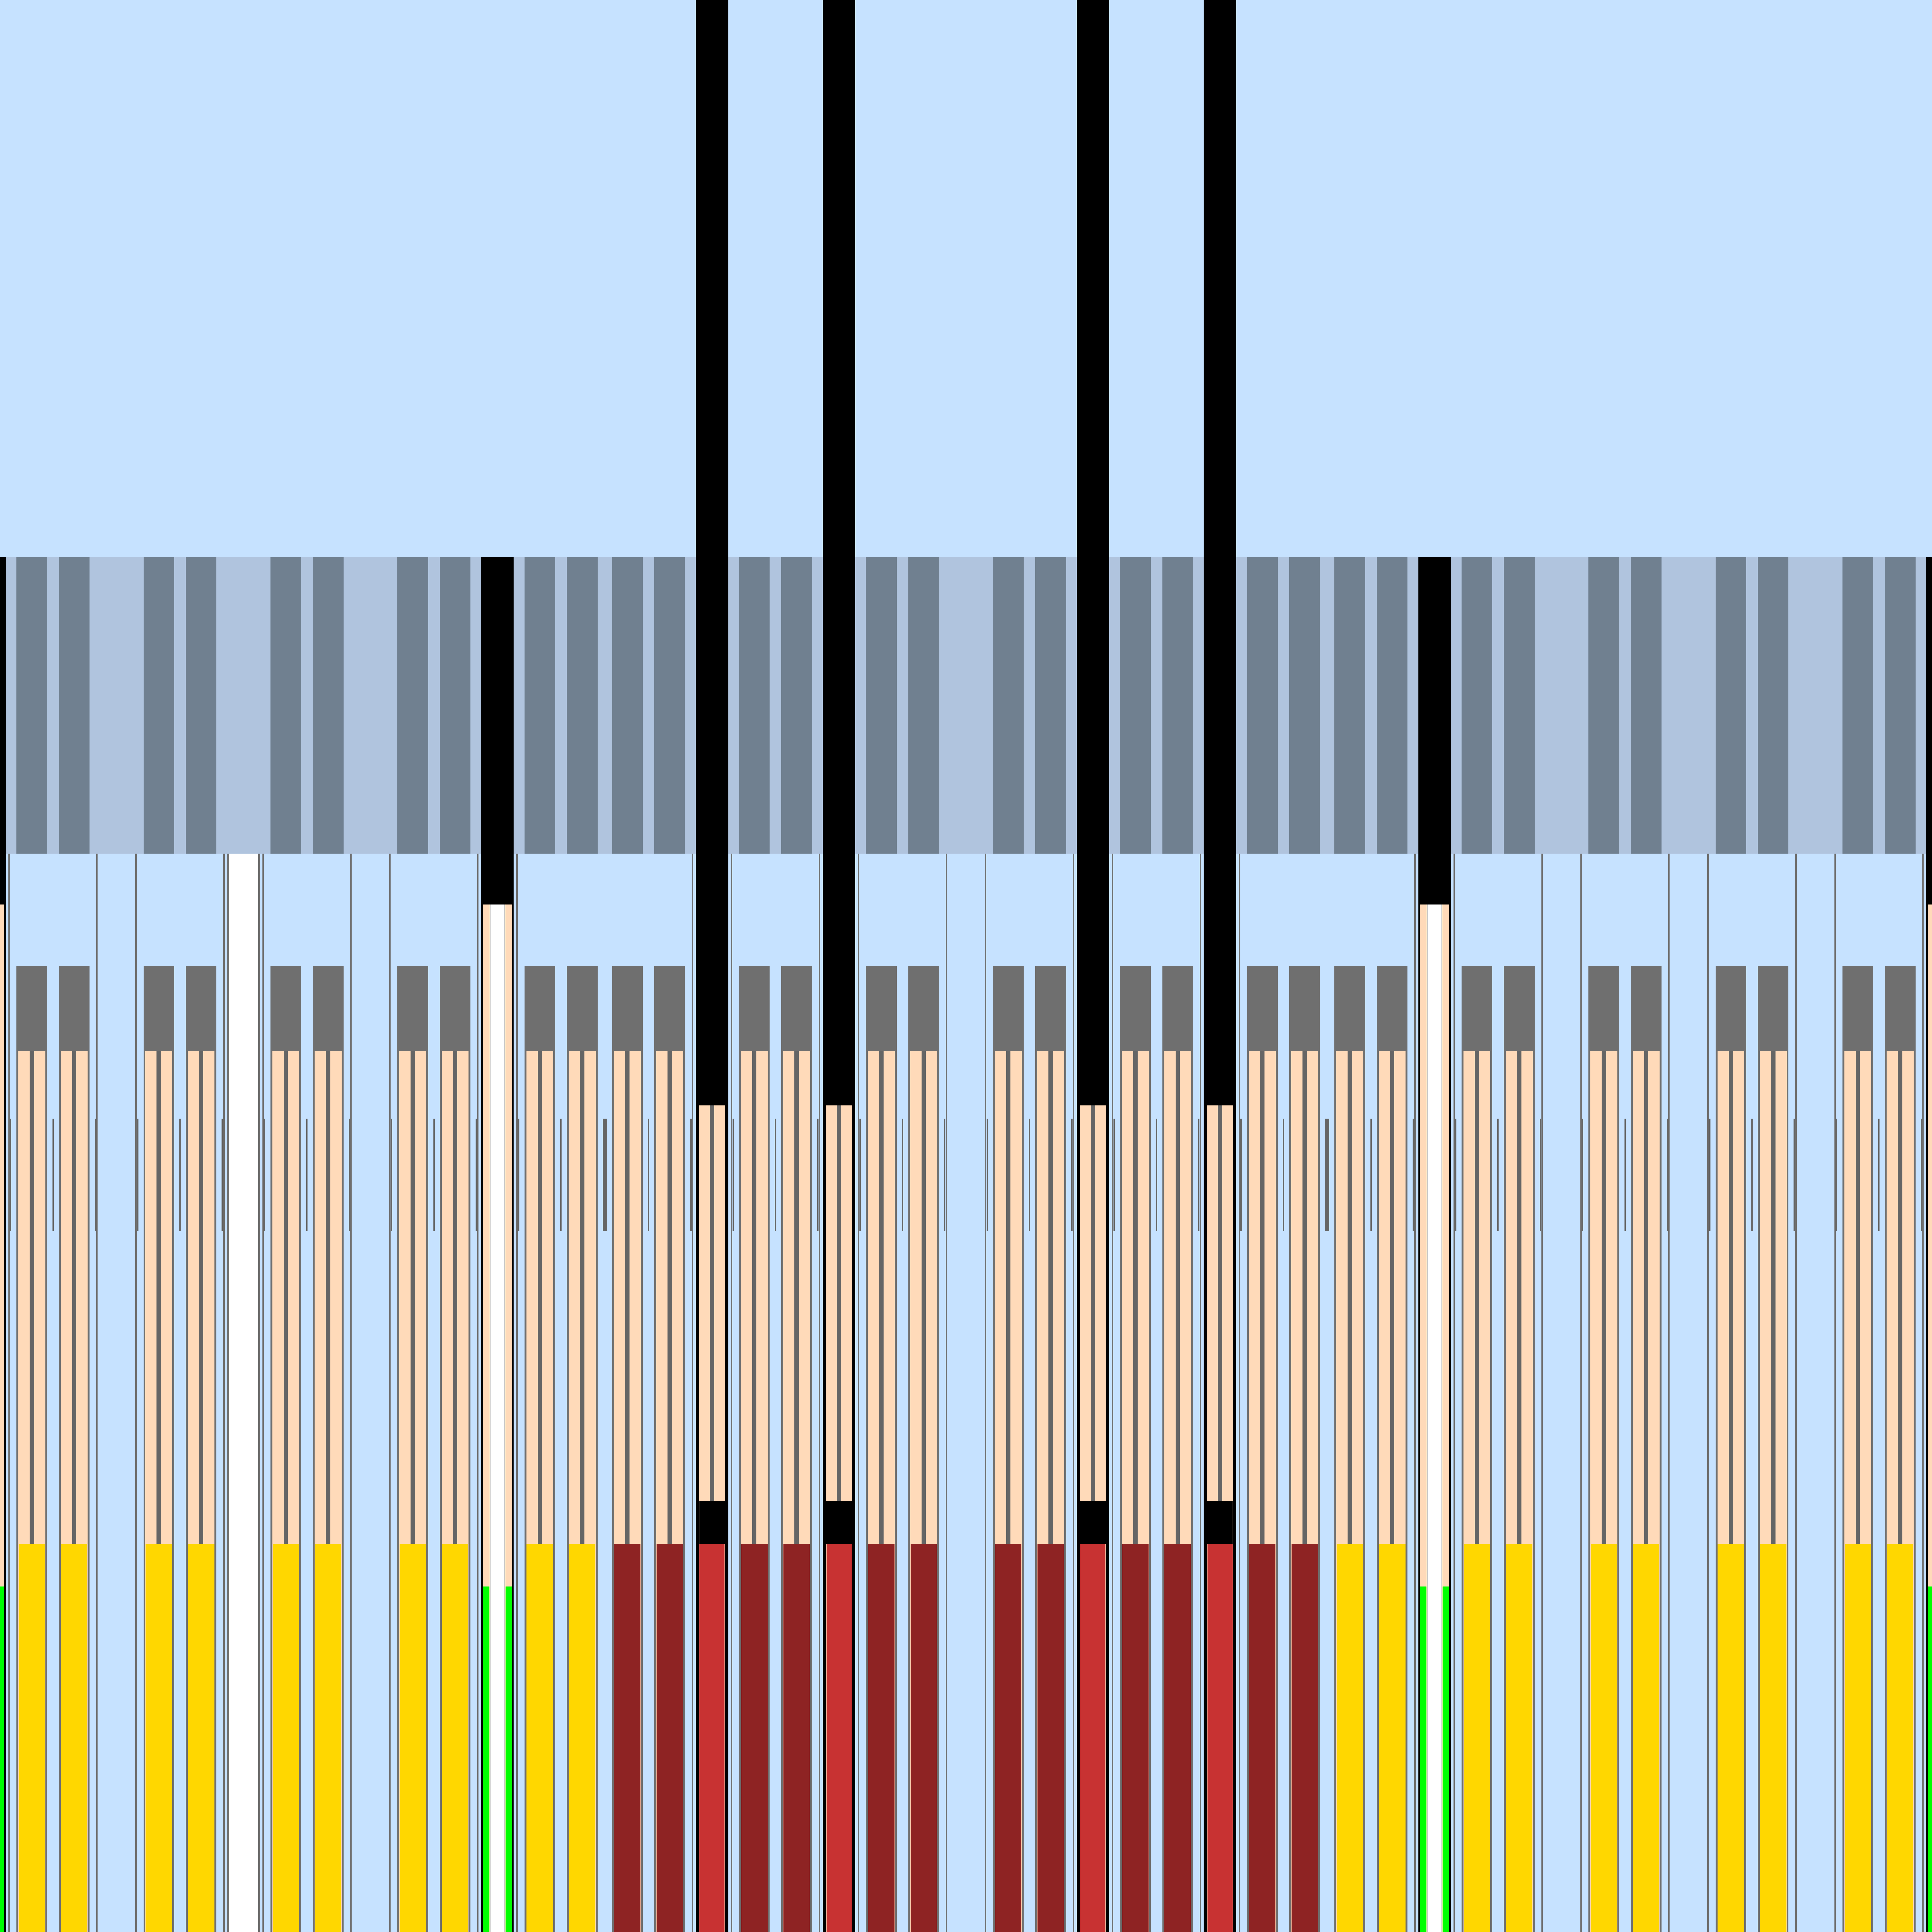
\includegraphics[height=\height cm]{specifications/axial/figs/axial_mats_row_8_topzoom.png}};
      \node[anchor=north] (dots) at (toppic.south) {$\vdots$};
      \node[anchor=north] (botpic) at (dots.south) {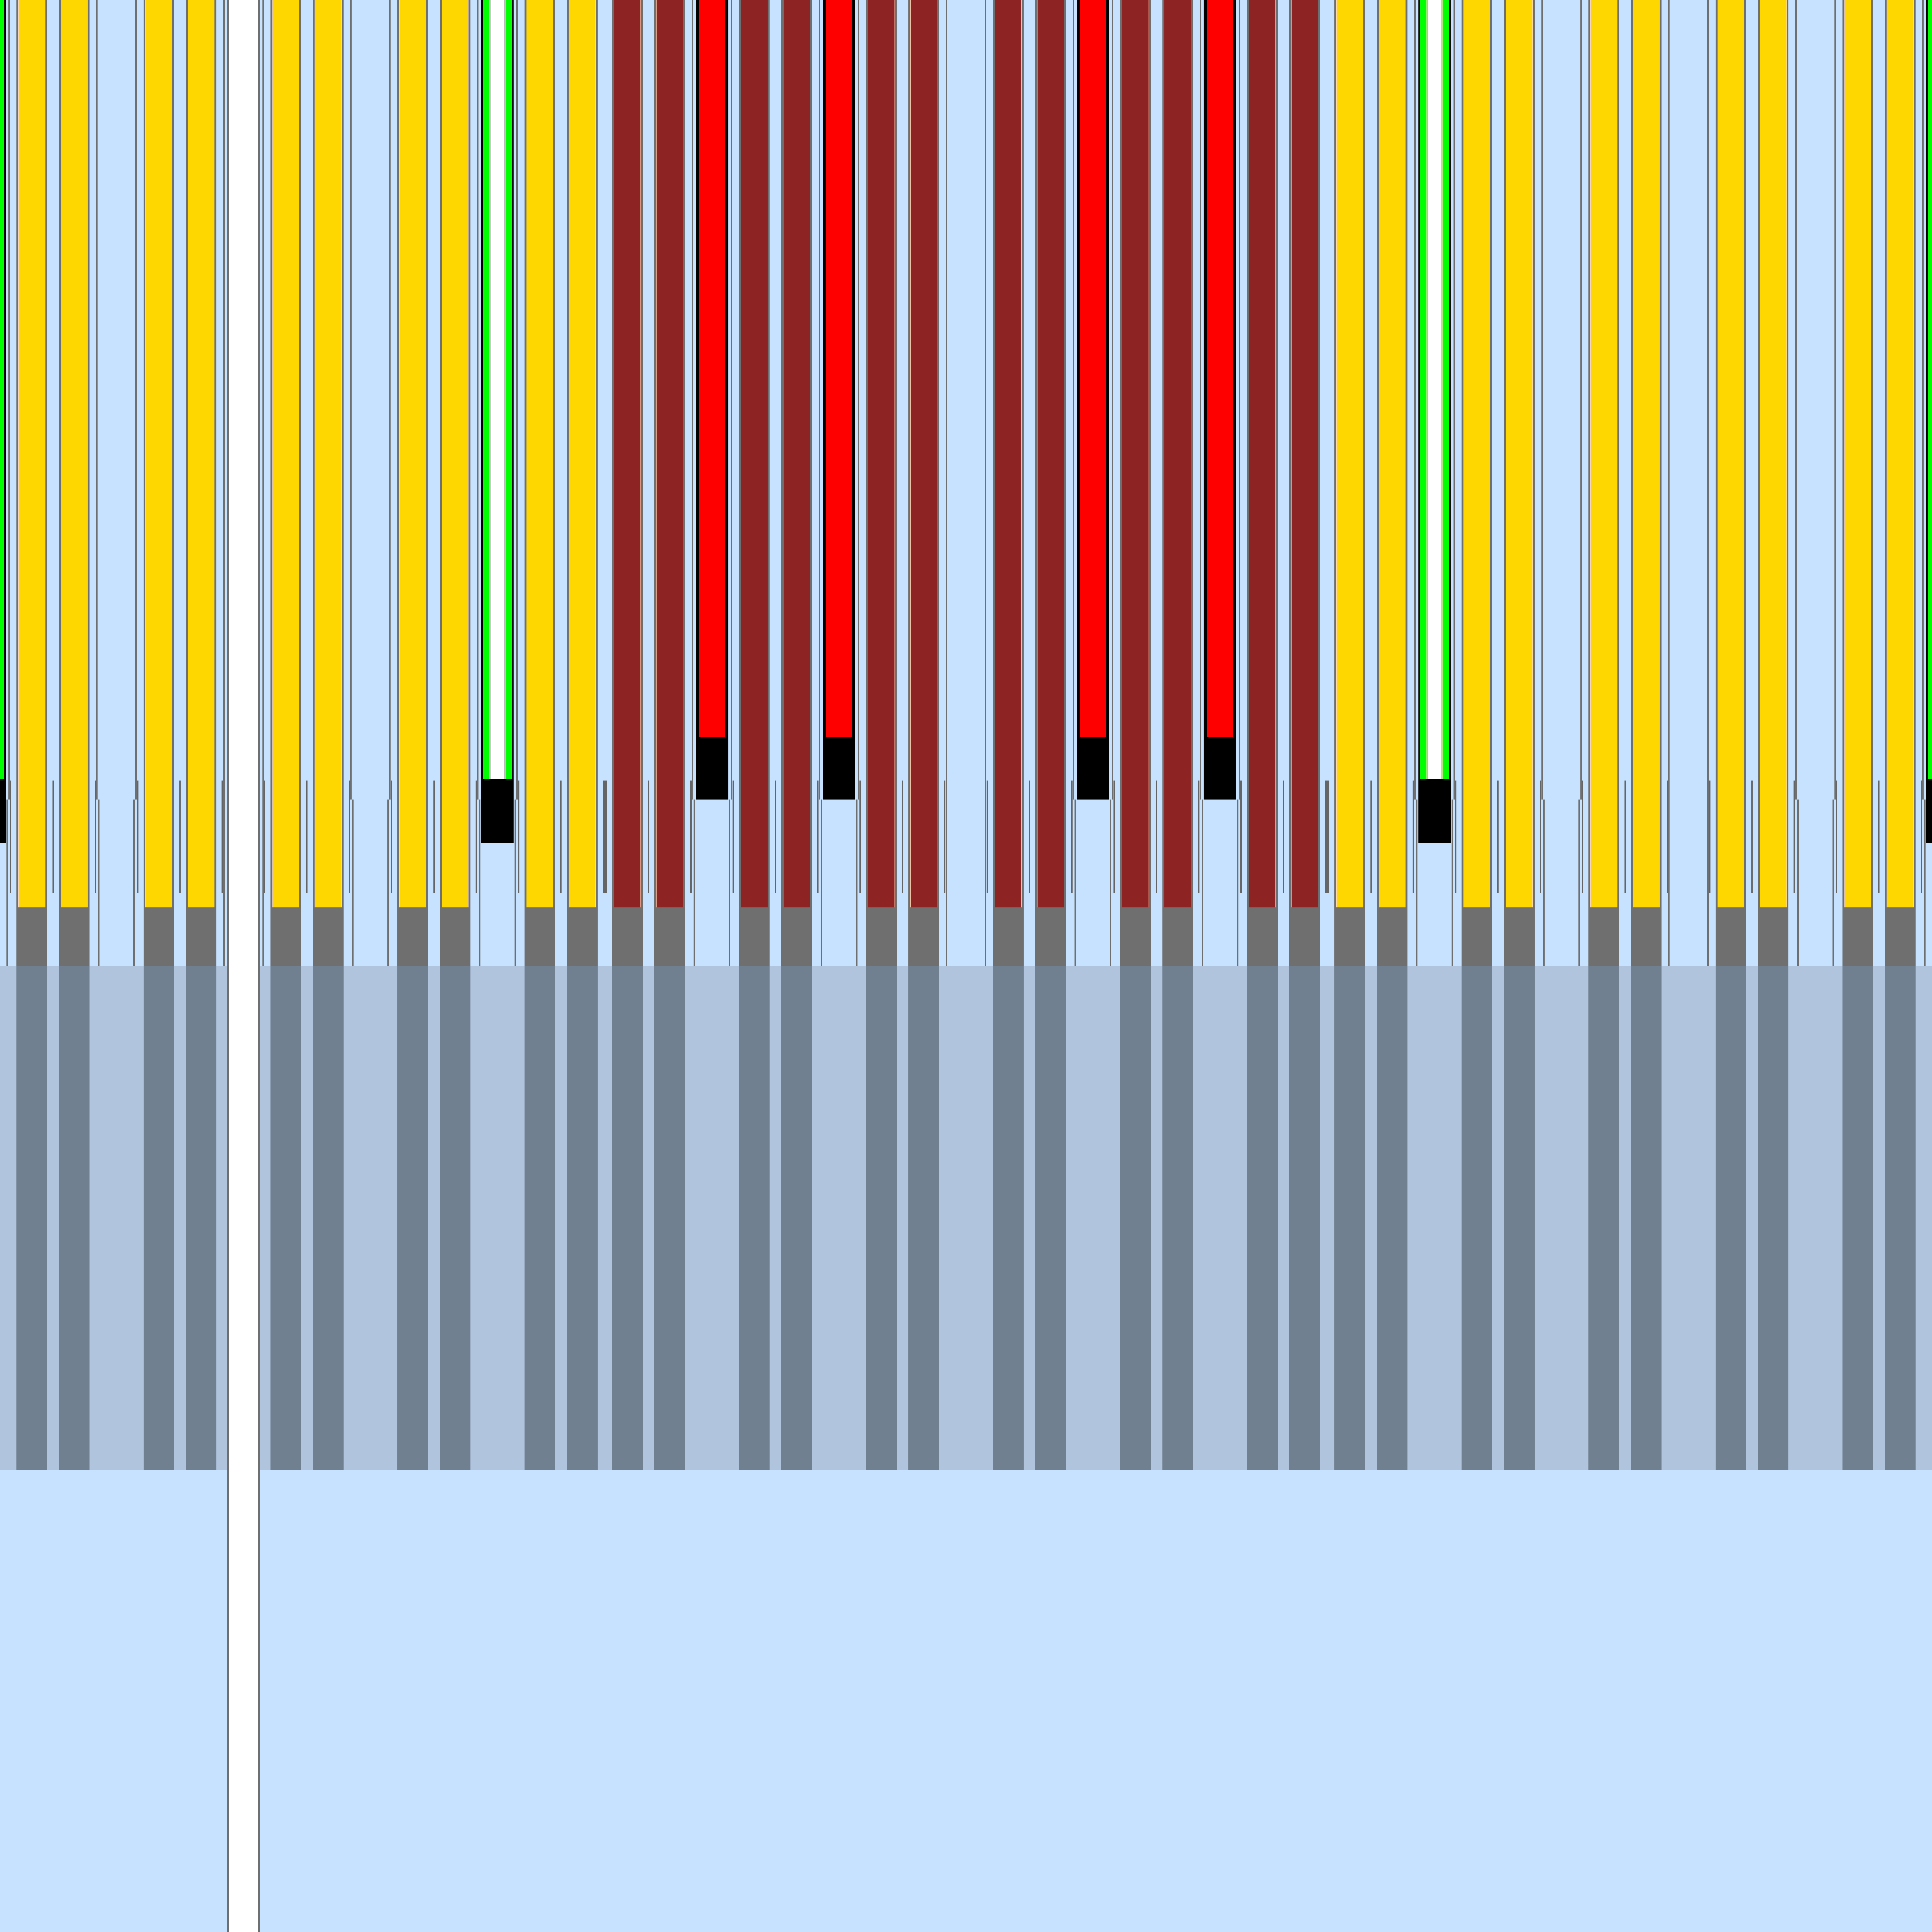
\includegraphics[height=\height cm]{specifications/axial/figs/axial_mats_row_8_botzoom.png}};

      % real geometries of the plots
      \def\realtopcenter{419.704}
      \def\realbotcenter{35.00}
      \def\realheight{57.5}
      
      \def\f{\height/\realheight}

      \def\n{20} % number of planes

      \foreach \a/\l/\c/\rc/\i in {20.0000/Bottom of Support Plate/botpic/\realbotcenter/1,
                            35.0000/Bottom of Fuel Rod/botpic/\realbotcenter/2,
                            36.7480/Bottom of Active Fuel/botpic/\realbotcenter/3,
                            37.1621/Grid 1 Bottom/botpic/\realbotcenter/4,
                            38.6600/Bottom of BPRA Rod/botpic/\realbotcenter/5,
                            39.9580/Bottom of Fully-Inserted RCCA Rod/botpic/\realbotcenter/6,
                            40.5200/Grid 1 Top/botpic/\realbotcenter/7,
                            40.5580/Bottom of BPRA Rod Absorber/botpic/\realbotcenter/8,
                            41.8280/Bottom of RCCA Rod Lower Absorber/botpic/\realbotcenter/9,
                            401.238/Top of BPRA Rod Absorber/toppic/\realtopcenter/10,
                            402.508/Top of Active Fuel/toppic/\realtopcenter/11,
                            403.778/Bottom of RCCA Rod Upper Plenum/toppic/\realtopcenter/12,
                            411.806/Grid 8 Bottom/toppic/\realtopcenter/13,
                            415.164/Grid 8 Top/toppic/\realtopcenter/14,
                            415.558/Top of RCCA Rod Upper Plenum/toppic/\realtopcenter/15,
                            417.164/Top of Fuel Rod Upper Plenum/toppic/\realtopcenter/16,
                            419.704/Top of Fuel Rod/toppic/\realtopcenter/17,
                            421.532/Top of BPRA Rod Upper Plenum/toppic/\realtopcenter/18,
                            423.049/Bottom of Upper Nozzle/toppic/\realtopcenter/19,
                            431.876/Top of Upper Nozzle/toppic/\realtopcenter/20
                            }
          \draw[red,thick] let \p{A}=(\c.west) in 
              (\x{A},\y{A}+\f*\a cm - \f*\rc cm) -- 
                  ++(\height+0.5,0) -- (\height/2+1.25,\i-\height*1.7) -- ++(0.75,0)
                      node[black,right,anchor=west,font=\scriptsize] {\l};

    \end{tikzpicture}
    
    \caption[Axial scale view of aggregate pincell model near core top and
    bottom]{Axial scale view of the model near the top and bottom of the fuel
    rods in row 8, showing pin plenums, approximated
    springs, end plugs, and structures. \emph{Blue}: water; \emph{orange}: helium;
    \emph{black}: stainless steel; \emph{dark gray}: Zircaloy; \emph{dim gray}
    Inconel; \emph{white}: air; \emph{slate gray}: nozzle / support plate
    stainless steel; \emph{steel blue}: nozzle / support plate borated water;
    \emph{green}: borosilicate glass; \emph{yellow}: fuel. \label{fig:tb_detail}}
\end{figure}
